\documentclass[12pt]{article}

\usepackage{graphicx}

%math
\usepackage{amsmath}

%%% Figures
\usepackage{caption}      % needed for subfigures
\usepackage{subcaption}   % needed for subfigures

%%% Colors are nice
\usepackage[dvipsnames]{xcolor}   % used for simple color names (e.g. "red")

%%% hyperref
\usepackage{hyperref}
\newcommand\myshade{85}
\colorlet{mylinkcolor}{black}
\colorlet{mycitecolor}{black}
\colorlet{myurlcolor}{Aquamarine}
\hypersetup{
  linkcolor  = mylinkcolor!\myshade!black,
  citecolor  = mycitecolor!\myshade!black,
  urlcolor   = myurlcolor!\myshade!black,
  colorlinks = true,
}

% Code
\usepackage{listings}

% Clever references need to be loaded after hyperref!
\usepackage[capitalize,nameinlink]{cleveref}       % used for clever references!

%%% Own commands
\newif\ifdebug

\newcommand{\todo}[1]{\ifdebug \textcolor{red}{\textit{\textbf{TODO:}} #1}\else \fi}    % for todos
\newcommand{\info}[1]{\ifdebug \textcolor{blue}{\textit{\textbf{INFO:}} #1}\else \fi}   % for infos
% \newcommand{\cc}[1]{\textcolor{DarkBlue}{\marginnote{\tiny #1}}}     % for comments in the margin

% nicer tables
\usepackage{booktabs}

%tikz party
\usepackage{tikz}

%supergmiadliche diagrams
\usepackage{smartdiagram}
% set the options
\smartdiagramset{%
  font=\normalsize,
  text width=25mm,
  arrow tip=to,
  uniform arrow color=true,
  arrow color=gray!50!black,
  border color=black,
  set color list={white,white,white}
}

% smaller gaps in enums
\usepackage{enumitem}
\setlist{nosep} % or \setlist{noitemsep} to leave space around whole list


\newtheorem{example}{Example}[section]
\newtheorem{theorem}[example]{Theorem}

\title{Combinatorial Pyramids – Development and Lessons Learned}
\author{David Pfahler}
\date{Technical Report for \\ \emph{Structural Pattern Recognition 2016W}}

%----------------------- Begin of Document -----------------------------------
%-----------------------------------------------------------------------------
\begin{document}

\debugtrue

%-----------------------------------------------------------------------------
%-----------------------------------------------------------------------------
\maketitle

\begin{figure}[!htb]
  \centering
  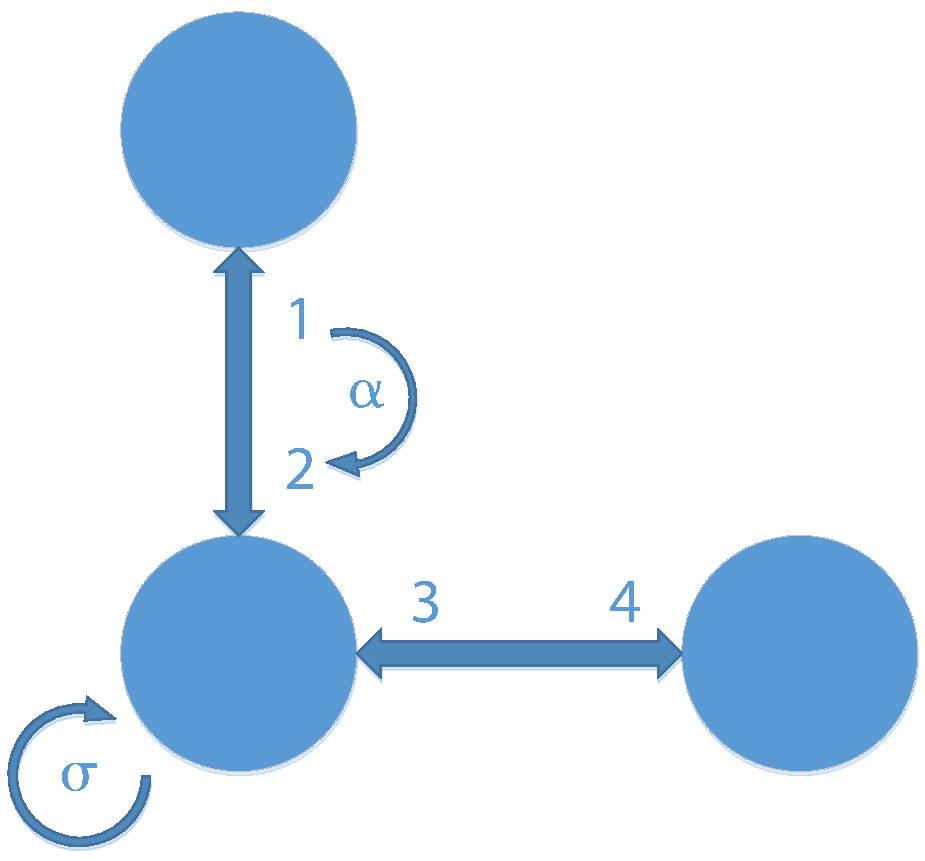
\includegraphics[width=0.3\textwidth]{img/combmap.pdf}
  \caption{A graph with labeled darts. \cref{tab:combmap} shows the involution \( \alpha \) of a dart and the permutation \( \sigma \).}\label{fig:combmap}
\end{figure}

\section{Introduction} % (fold)
\label{sec:introduction}

\subsection{Lecture} % (fold)
\label{sub:lecture}

I wrote this work for the lecture \emph{Structural Pattern Recognition} in the \emph{WS 2016/17}. The content of the lecture was:
\begin{itemize}
  \item Relations between patterns in space and time
  \item Representing structure: strings, arrays, trees, graphs, maps and grammars
  \item Shape and context, embedding in an n-dimensional space
  \item Distances on a given structure graph spectra and eccentricity
  \item Operations on structures and among structures: recognition, parsing
  \item Exact and inexact matching
  \item Modification of structure under motion and tracking
  \item Topology (nD holes, persistence) applications.
\end{itemize}

As my lab exercise in structural pattern recognition I chose the topic ``\emph{Combinatorial Pyramids}'' from the lecture unit 5. To intensify my knowledge from the associated lecture by means of practical examples.

% subsection lecture (end)

\subsection{Problem Specification} % (fold)
\label{sub:problem}

To describe the content of an image it is necessary to extract the objects that an image shows.
The positions of the identified objects to each other gives important information of the context of the image.
An image is most commonly represented by an array of pixels.
To understand the context of the image, it needs to be partitioned into regions.
The context of this regions is called the Region Adjacency Graph (RAG).
\par
To create the RAG the pixel array of the image needs to be transformed into a graph representation.
This is a computational expensive process, because in contrast to the implicit representation in the system memory of a pixel array, a graph representation needs to save pointers for the darts to the nodes (which are the pixels) of the image.
\par
The Combinatorial Map (CM) supports an efficient way to represent the darts in the system memory.
Additionally it enables the application of the graph operations to \emph{contract} and \emph{remove} a dart.

% subsection problem (end)

\begin{table}[tb]
  \caption{Involution and permutation of the CM from \cref{fig:combmap}}\label{tab:combmap}
  \centering

  \begin{tabular}{lcccc}
  & \textbf{1} & \textbf{2} & \textbf{3} & \textbf{4} \\
  \midrule
     \( \alpha \)& 2 & 1 & 4 & 3\\
     \( \sigma \)& 4 & 2 & 3 & 1\\
  \bottomrule
  \end{tabular}
\end{table}

\subsection{Outline} % (fold)
\label{sub:outline}

In the \cref{sec:development_methodology} I introduced the literature research (\cref{sub:related_work}) and I present the pre-work I did to understand the CM (\cref{sub:python_implementation}).
In the \cref{sec:computation_of_the_dart_values,sec:construction_of_the_initial_cm_level,sec:construction_of_the_pyramid} the \texttt{MATLAB} implementation is described in detail and in \cref{sec:results} I present the results.

% subsection outline (end)

% section introduction (end)

\section{Development methodology} % (fold)
\label{sec:development_methodology}

\subsection{Related work} % (fold)
\label{sub:related_work}

\begin{figure}[tb]
  \centering

  \begin{subfigure}[b]{0.25\textwidth}
        \includegraphics[width=\textwidth]{img/prip1}
        \caption{}\label{fig:prip1}
    \end{subfigure}
    ~
    \begin{subfigure}[b]{0.25\textwidth}
        \includegraphics[width=\textwidth]{img/prip2}
        \caption{}\label{fig:prip2}
    \end{subfigure}
    ~
    \begin{subfigure}[b]{0.4\textwidth}
        \includegraphics[width=\textwidth]{img/prip3}
        \caption{}\label{fig:prip3}
    \end{subfigure}

    \begin{subfigure}[b]{0.4\textwidth}
        \includegraphics[width=\textwidth]{img/combine_remove.jpg}
        \caption{}\label{fig:combine_remove}
    \end{subfigure}

  \caption{(a) an input image. (b) the segmented image at the first level. (c) the top level of the combinatorial pyramid. (d) Combine and remove operations on a graph}\label{fig:prip}
\end{figure}

\cite{torrescanonical} is a Technical Report about operations
on a Combinatorial Pyramid (CP)

Recap: Operations on a Combinatorial Map (CM):
Remove
Contract

\cite{brun2001introduction} is an introduction to the CP. With
background information an the contraction
kernel.

Recap: Contraction Kernel

\begin{figure}[tb]
  \centering

  \begin{subfigure}[b]{0.2\textwidth}
      \includegraphics[width=\textwidth]{img/contract_kernel1}
      \caption{}\label{fig:contract_kernel1}
  \end{subfigure}
  ~
  \begin{subfigure}[b]{0.2\textwidth}
      \includegraphics[width=\textwidth]{img/contract_kernel2}
      \caption{}\label{fig:contract_kernel2}
  \end{subfigure}
  ~
  \begin{subfigure}[b]{0.2\textwidth}
      \includegraphics[width=\textwidth]{img/contract_kernel3}
      \caption{}\label{fig:contract_kernel3}
  \end{subfigure}
  ~
  \begin{subfigure}[b]{0.2\textwidth}
      \includegraphics[width=\textwidth]{img/contract_kernel4}
      \caption{}\label{fig:contract_kernel4}
  \end{subfigure}

  \begin{subfigure}[b]{0.2\textwidth}
      \includegraphics[width=\textwidth]{img/contract_kernel5}
      \caption{}\label{fig:contract_kernel5}
  \end{subfigure}
  ~
  \begin{subfigure}[b]{0.2\textwidth}
      \includegraphics[width=\textwidth]{img/contract_kernel6}
      \caption{}\label{fig:contract_kernel6}
  \end{subfigure}
  ~
  \begin{subfigure}[b]{0.2\textwidth}
      \includegraphics[width=\textwidth]{img/contract_kernel7}
      \caption{}\label{fig:contract_kernel7}
  \end{subfigure}
  ~
  \begin{subfigure}[b]{0.2\textwidth}
      \includegraphics[width=\textwidth]{img/contract_kernel8}
      \caption{}
      \label{fig:contract_kernel8}
  \end{subfigure}

  \caption{The creation of a contraction kernel}
  \label{fig:creationg_of_a_kernel}
\end{figure}

\cite{brun2003contraction} describes contraction in parallel with
contraction kernels

Recap: Problem why parallel
contraction/removal is not trivial

% subsection related_work (end)

\subsection{Python implementation} % (fold)
\label{sub:python_implementation}

I Implemented a simple python class for CM
Not for computations but for representations

\begin{lstlisting}[language=Python]
import CombinatorialMap
map = CombinatorialMap()
map.setSize(5, 5)
map.printNodes()
\end{lstlisting}

Also created functions to receive:
All darts with specific direction
All involutions of specific darts
The orbit of a vertex
All next darts
…

These are used to understand and create a
CM from an image
% subsection python_implementation (end)

% section development_methodology (end)

\section{Computation of the dart values} % (fold)
\label{sec:computation_of_the_dart_values}

\begin{figure}[tb]
  \centering

  \begin{subfigure}[b]{0.46\textwidth}
        \includegraphics[width=\textwidth]{img/values_init.jpg}
        \caption{}\label{fig:dart_values_init}
    \end{subfigure}
    ~
    \begin{subfigure}[b]{0.45\textwidth}
        \includegraphics[width=\textwidth]{img/values_new.jpg}
        \caption{}\label{fig:dart_values_news}
    \end{subfigure}

  \caption{\todo{caption}}\label{fig:dart_values}
\end{figure}

A dart in an image is a transition from one pixel to
another.
Compute from every pixel the change of the pixel
value to every neighbor (N,E,S,W)

% section computation_of_the_dart_values (end)

\section{Construction of the initial CM level} % (fold)
\label{sec:construction_of_the_initial_cm_level}

\subsection{Computation of the dart indices} % (fold)
\label{sub:computation_of_the_dart_indices}

Computation of the dart indices
Example South Indices:
Added by 4 inside the image. On the border it
is only added by 3 (because the west dart is
missing)
Also exceptions in the first row and the last
row (missing north dart)
Additional exceptions for the corners

% subsection computation_of_the_dart_indices (end)

\subsection{Computation of the next index} % (fold)
\label{sub:computation_of_the_next_index}

Computation of the next index:
one row:
\begin{lstlisting}[language=Matlab]
repmat([2; 2; -1; -3], width-2, 1)
\end{lstlisting}
middle of the image:

\begin{lstlisting}[language=Matlab]
repmat([next_darts_one_row; 1; 1; -2; 2; -1; -1],height-2, 1)
\end{lstlisting}

Special cases for first and last row

% subsection computation_of_the_next_index (end)

\subsection{Computation of the other properties} % (fold)
\label{sub:computation_of_the_other_properties}

Involution \( \alpha \)

Previous Dart \( \rho \)

\begin{lstlisting}[language=Matlab]
cm.involution(N) = S
cm.involution(E) = W

cm.prev(cm.next) = 1:num_darts
\end{lstlisting}


% subsection computation_of_the_other_properties (end)

% section construction_of_the_initial_cm_level (end)

\section{Construction of the pyramid} % (fold)
\label{sec:construction_of_the_pyramid}

\begin{figure}[tb]
\centering
\smartdiagram[circular diagram:clockwise]
{
  Contract Darts (\cref{sub:contraction}),
  Simplify Level (\cref{sub:simplification}),
  Compute Contraction Kernel (\cref{sub:compute_the_contraction_kernel})
}
\caption{The creation loop of the pyramid}%
\label{fig:creation loop}
\end{figure}

\subsection{Compute the contraction kernel} % (fold)
\label{sub:compute_the_contraction_kernel}

\begin{figure}[tb]
  \centering
  \vspace{-10 mm}

  \begin{subfigure}[b]{0.15\textwidth}
      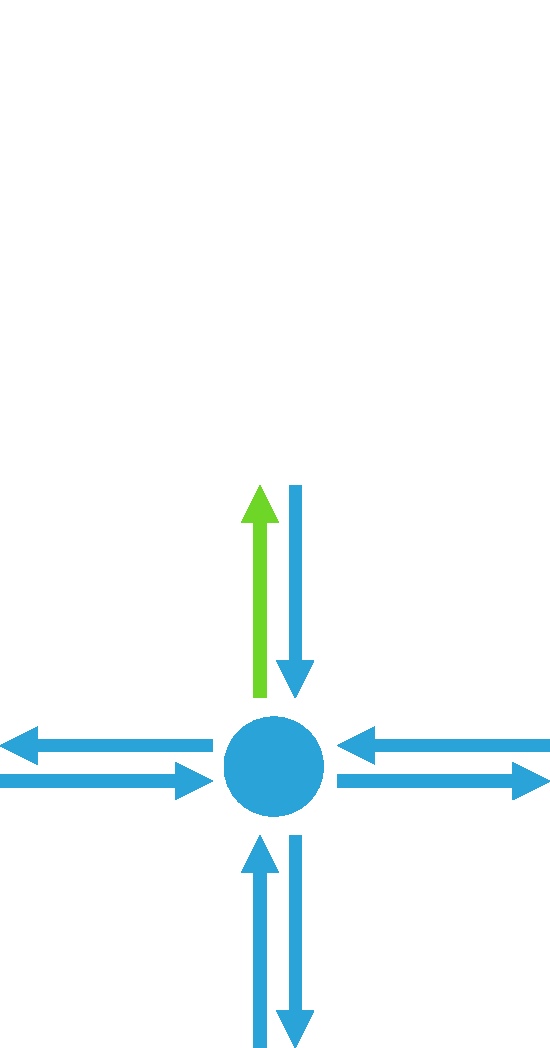
\includegraphics[width=\textwidth]{img/1}
      \caption{}\label{fig:contraction_kernel_greedy1}
  \end{subfigure}
  ~
  \begin{subfigure}[b]{0.15\textwidth}
      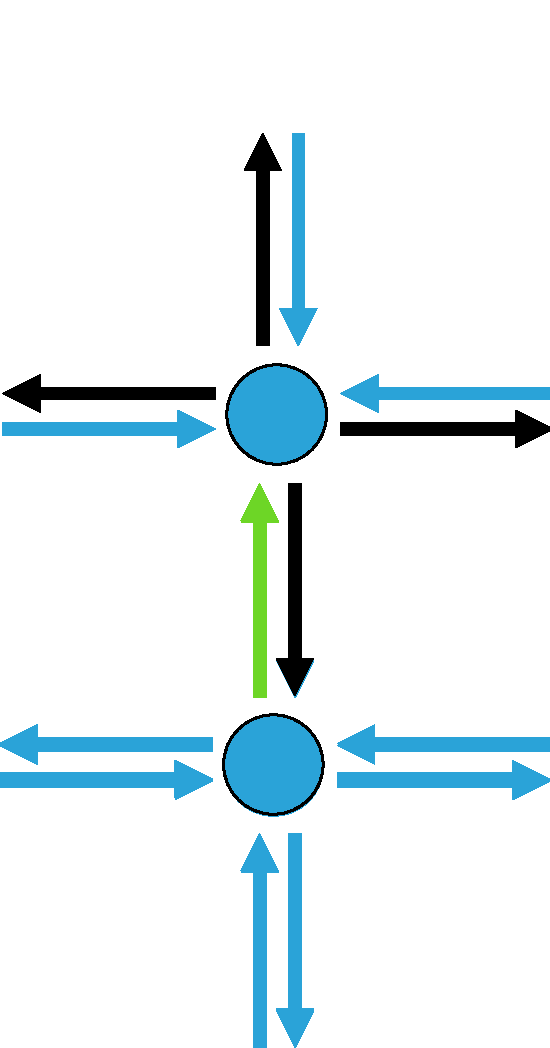
\includegraphics[width=\textwidth]{img/2}
      \caption{}\label{fig:contraction_kernel_greedy2}
  \end{subfigure}
  ~
  \begin{subfigure}[b]{0.15\textwidth}
      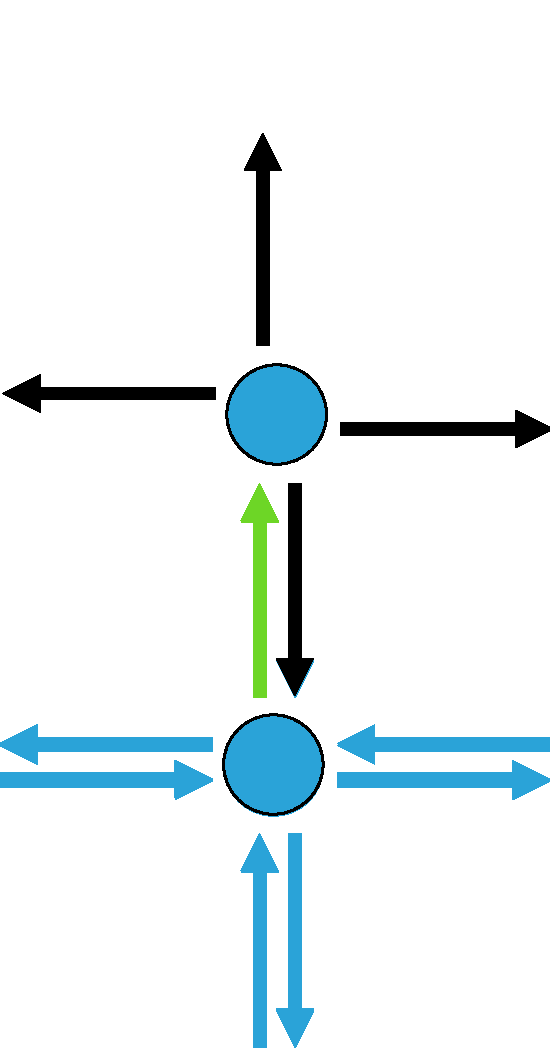
\includegraphics[width=\textwidth]{img/3}
      \caption{}\label{fig:contraction_kernel_greedy3}
  \end{subfigure}
  ~
  \begin{subfigure}[b]{0.15\textwidth}
      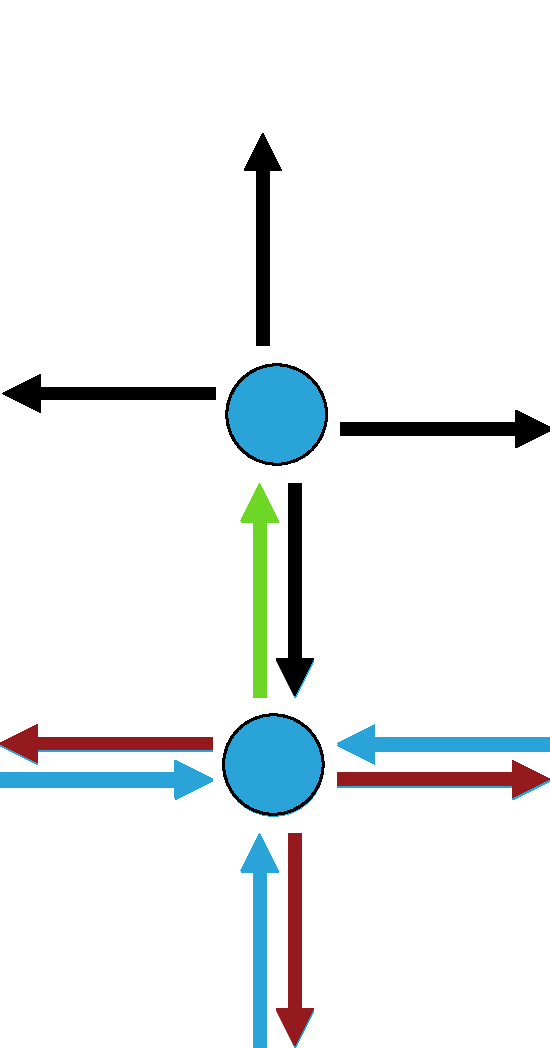
\includegraphics[width=\textwidth]{img/4}
      \caption{}\label{fig:contraction_kernel_greedy4}
  \end{subfigure}
  ~
  \begin{subfigure}[b]{0.15\textwidth}
      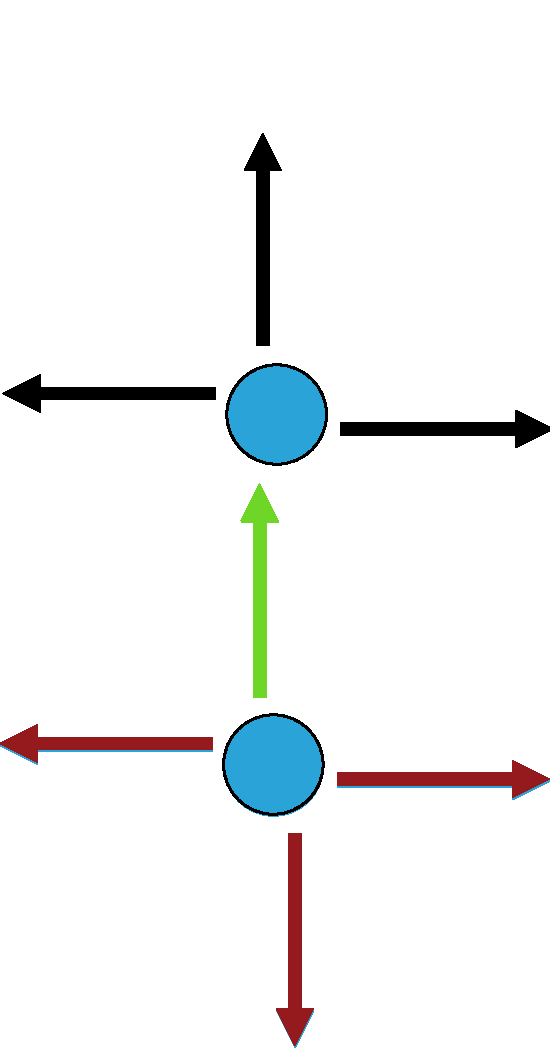
\includegraphics[width=\textwidth]{img/5}
      \caption{}\label{fig:contraction_kernel_greedy5}
  \end{subfigure}

  \caption{(a) Assign next best dart for CK (b) Get the involution of the dart and the orbit of the involution (c) now remove the involution of the involution orbit from the set of valid darts (d) now get the orbit of the dart (e) And remove its involution}
  \label{fig:contraction_kernel_greedy}
\end{figure}

Sort the darts by its values
Add dart to contraction kernel if:

Exceptions:
Self loops
Pending edges

\begin{figure}[tb]
  \centering

    \begin{subfigure}[t]{0.3\textwidth}
      \includegraphics[width=\textwidth]{img/contract2.jpg}
      \caption{}\label{fig:dart_contract2}
    \end{subfigure}
    ~
    \begin{subfigure}[t]{0.3\textwidth}
      \includegraphics[width=\textwidth]{img/contract3.jpg}
      \caption{}\label{fig:dart_contract3}
    \end{subfigure}
    ~
    \begin{subfigure}[t]{0.3\textwidth}
      \includegraphics[width=\textwidth]{img/contract1.jpg}
      \caption{}\label{fig:dart_contract1}
    \end{subfigure}
  \caption{\todo{caption}}\label{fig:dart_contract}
\end{figure}

% subsection compute_the_contraction_kernel (end)

\subsection{Contraction} % (fold)
\label{sub:contraction}

Recap: Contract Darts

\begin{align}
  \sigma'(\rho(x))   &:= \sigma(-x)    \\
  \sigma'(\rho(-x))  &:= \sigma(x)     \\
  \rho'(\sigma(x))   &:= \rho(-x) \\
  \rho'(\sigma(-x))  &:= \rho(x)
\end{align}

% subsection contraction (end)

\subsection{Simplification} % (fold)
\label{sub:simplification}

\begin{figure}[tb]
  \centering
  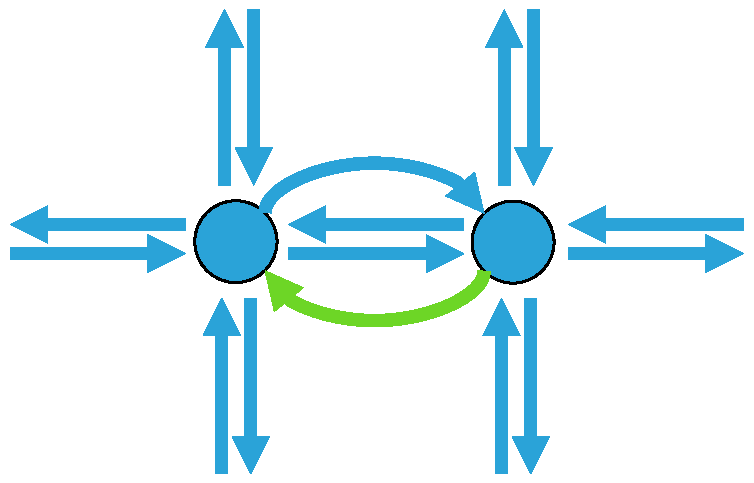
\includegraphics[width=0.6\textwidth]{img/face.pdf}
  \caption{The number of darts of this face is less than 2 and it can be removed}
  \label{fig:faces}
\end{figure}

When contracting darts double edges and self-direct-loops are created. By removing these darts the pyramid is easier to read.
\todo{faster to compute check}

Check if the face of a dart \(x\) has less than 2 darts:

\begin{itemize}
  \item Get the involution \(\alpha(x)\)
  \item Get the previous of the involution of the dart \(\rho(\alpha(x))\)
  \item add this to the face and repeat for this dart until the initial dart is reached
\end{itemize}

Special cases for removal:
Self-Direct-Loops (2 cases)

\begin{figure}[tb]
  \centering

    \begin{subfigure}[b]{0.3\textwidth}
      \includegraphics[width=\textwidth]{img/simply2.jpg}
      \caption{}\label{fig:dart_simply2}
    \end{subfigure}
    ~
    \begin{subfigure}[b]{0.3\textwidth}
      \includegraphics[width=\textwidth]{img/simply3.jpg}
      \caption{}\label{fig:dart_simply3}
    \end{subfigure}
    ~
    \begin{subfigure}[b]{0.3\textwidth}
      \includegraphics[width=\textwidth]{img/simply1.jpg}
      \caption{}\label{fig:dart_simply1}
    \end{subfigure}
  \caption{\todo{caption}}\label{fig:dart_simply}
\end{figure}

% subsection simplification (end)

% section construction_of_the_pyramid (end)

\section{Results} % (fold)
\label{sec:results}

% section results (end)

%-----------------------------------------------------------------------------
\bibliographystyle{abbrv}
\bibliography{bibliography}


\end{document}
